\chapter{Experimental Setup}
\label{chap:setup}

Knowledge about the components and techniques required for optimizing order placement was provided in Chapter \ref{chap:preliminaries}, and previous approaches were introduced in Chapter \ref{chap:related-work}.
The process of collecting historical event data and the construction of a limit order book was explained in Chapter \ref{chap:data}.
The data was investigated and theories were stated as a guideline for a future learning process.
However, in order to apply reinforcement learning, an environment has to be developed which is flexible enough to allow investigation regarding different types of features and learning algorithms that are incorporated in an agent.
The correctness of such an environment is critical as it emulates a stock exchange and therefore determines how orders would have been transacted in the past.
If the implementation varies from the one used in exchanges, or does not cover certain edge cases, the matching of placed orders would differ significantly from the one in a production setup.

This chapter aims to build an environment that emulates a subset of the capabilities of a real world exchange in order to determine how limit orders would have been processed, had they been placed at a given point in time in the past.
Therefore, the setup of the environment is described at first and explains how the required components work in combination such that a learner can simulate order placement.
Additionally, an extension of this environment is provided
to simulate simultaneous order placement on both sides of the book.
This process is commonly referred to as \textit{market making}.
Subsequently, feature engineering is described which incorporates previously stated theories and results in features that can be used by the agents.
Finally, two implementations of reinforcement learning agents are provided.
A Q-Learning agent will serve as the learner when no market variables are provided and a Deep Q-Network agent is developed to handle complex features.


\section{Order Placement Environment}

The execution environment serves as the main reinforcement learning environment (see Section \ref{sec:rl-environment}) and allows to investigate the behaviour of order placement on a historical data set. 
Therefore, the previously described components which were introduced in Chapter \ref{chap:preliminaries} come into play.
The main idea is that the environment allows an agent to observe a state in the order book space and respond with a limit level on where to place its order in the order book at that moment in time.
The task of the environment is then to evaluate the outcome of this order placement and report to the agent accordingly.

OpenAI Gym \cite{brockman2016openai} is an open source toolkit for reinforcement learning.
The interfaces of this toolkit were used in order to follow their standards while building this environment.
The advantage of which is that any OpenAI Gym compatible agent and bench-marking tools can make use of this environment.

\subsection{Overview of components}

\begin{figure}[H]
    \centering
    \makebox[\linewidth]{
        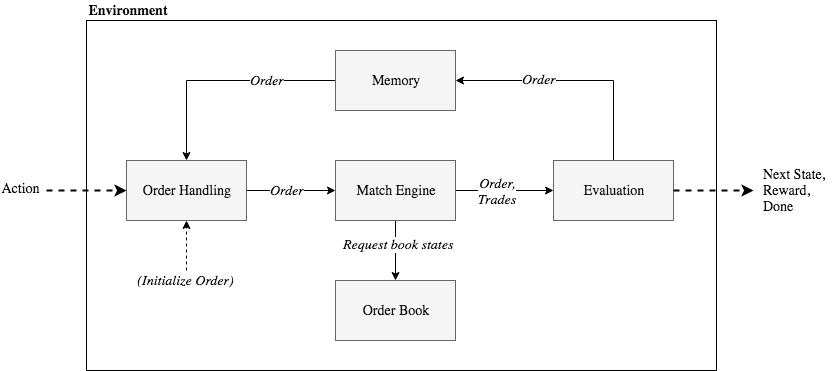
\includegraphics[width=14cm]{images/rl-env-overview}
    }
    \caption{Overview of reinforcement learning order placement environment.}
    \label{fig:rl-env-overview}
\end{figure}

Figure \ref{} shows this process in greater detail.

\subsection{Configuration parameters}

In order for the environment to be flexible and handle various attempts of placing orders, configuration parameter have to be defined.


\subsection{State}
Unlike in most traditional reinforcement learning environments, each step taken by the agent leads to a complete change of the state space.
Consider a chess board environment, where the state space is the board equipped with figures. 
After every move taken by the agent, the state space would look exactly the same, except of the figure moved with that step. 
This process would go on until the agent either wins or looses the game and the state space would be reset to the very same as in the beginning of the previous epoch.

In this environment, however, the state space is defined by all the possible sequences of states an agent can take in order to fully execute all the inventory.
If market variables are used as features, the state space increases drastically due to the initialization using a random order book state and (2) the fact that orders will match according to what is listed in the order book states that are processed by the match engine.
Hence, for each step taken by the agent, the order book states are likely to be different and thus the state the agent observes changes equally. 
It is, as if not only one or two figures of the chess board change their position, but almost all of them.

What the agent effectively observes depends on provided feature set (see Section \ref{sec:feature-engineering} below), that results in some state $s \in R^d$.

\subsection{Action}

A discrete action space represented by a vector of size equal to the number of limit levels ($l \in L$) is configured. 
The action space features actions $a \in Z$ which represent the limit level segmented in \$0.10 steps.
That is, $l_i = p_m + i * 0.1$, whereas $p_m$ is the market price at the time the order was placed.
The action space is configurable and the default implementation is of size 101, indicating the limit levels starting at -50 up to +50.
Negative limit levels indicate the listing deep in the book and positive listings relate to the level in the opposing side of the book.
In the default case that is, $p_m - 5.0$ to $p_m + 5.0$. 
Thus, at each time-step $t$ the agent selects an action $a_t$ from the set of legal actions, $A = {l_{min}, . . . , l_{max}}$, whereas $l_{min}$ is the most negative limit level and $l_{max}$ is the most positive limit level.

\subsection{Reward}

The reward is defined as the difference of the market price before the order was placed and the volume weighted average price (Eq. \ref{eq:vwap}) paid or received after the order has been filled. 
Hence, for buying assets the reward is defined as $R=p_{T}-p_{vwap}$ and for selling assets $R=p_{vwap}-p_T$, whereas $p_T$ is the market price at time step $t=T$.
Given the definition of the discounted return (Eq. \ref{eq:discounted-return}) we calculate $R_t=\sum_{t'=t}^{t_0}{\gamma^{t'-t}*r_{t'}}$, where $t_0$ is the time step at which the agent has its time horizon for the ongoing order fully consumed.

\section{Market making Environment}

\section{Feature engineering}
\label{sec:feature-engineering}


\section{Q-Learning agent}

One of the reinforcement learning algorithms used in this work is known as \textit{Q-Learning}. 
The name derives from the application of the previously presented Q-function (Eq. \ref{eq:q-function}), more specifically its use within the Bellman equation (\ref{eq:bellman}) that undergoes an iterative update.
\\
\\
The general idea is ... 

\section{Deep Q-Network agent}
